\documentclass[]{article}
\usepackage{amssymb}
\usepackage{amsmath}
\usepackage[utf8]{inputenc}
\usepackage{graphicx}
\usepackage{booktabs}
\usepackage{listings}
\usepackage{color}
\usepackage{tabularx}
\usepackage{hyperref}

\definecolor{dkgreen}{rgb}{0,0.6,0}
\definecolor{gray}{rgb}{0.5,0.5,0.5}
\definecolor{mauve}{rgb}{0.58,0,0.82}

\lstset{frame=tb,
	%language=C++,
	aboveskip=3mm,
	belowskip=3mm,
	showstringspaces=false,
	columns=flexible,
	basicstyle={\small\ttfamily},
	numbers=none,
	numberstyle=\tiny\color{gray},
	keywordstyle=\color{blue},
	commentstyle=\color{dkgreen},
	stringstyle=\color{mauve},
	breaklines=false,
	breakatwhitespace=true,
	tabsize=2
}


\title{FYS-STK4155 H20 - Project 1:\\An assessment of OLS, Ridge and LASSO Regression on Areally Distributed Data}
\author{Olav Fønstelien}

\begin{document}
\maketitle

\begin{abstract}
%The abstract gives the reader a quick overview of what has been done and the most important results. Try to be to the point and state your main findings. It could be structured as follows 
% - Short introduction to topic and why its important 
% - Introduce a challenge or unresolved issue with the topic (that you will try to solve) 
% - What have you done to solve this 
% - Main Results 
% - The implications
In this report I evaluate the OLS, Ridge and LASSO regression methods on aerially distributed data. Regression methods are powerful tools for data analysis and modeling, and I show in this report that these methods may reveal underlying truths about sampled data, specifically a quantification of the data's error or noise, and equally useful a model for simulating unseen data. This is shown first in a controlled manner on simulated data with known error using the Franke function. Then on geological data representing altitude above sea level of a mountain range. I show that for small data sets, Ridge and LASSO may give better estimates of these data, while for larger data sets, where the number of predictors is much smaller than the number of samples, OLS is preferrable.

For background material and source files, visit my github repo at \url{https://github.com/fonstelien/FYS-STK4155/tree/master/project1}.

\end{abstract}

\section{Introduction} \label{intro}
%When you write the introduction you could focus on the following aspects
% - Motivate the reader, the first part of the introduction gives always a motivation and tries to give the overarching ideas
% - What I have done
% - The structure of the report, how it is organized etc
OLS, Ridge and LASSO are three popular methods for linear regression. They are related to each other in that Ridge and LASSO (least absolute shrinkage and selection operator) are refinements of OLS (ordinary least squares). They aim to \textit{shrink} the coefficient estimates $\mathbf{\hat{\beta}} \in \mathbb{R}^p$ towards zero by penalizing their value and hence reducing their variance \cite{james2013introduction}.

In this report we will study each of these methods and how they perform when they are applied on $n$th degree polynomial fit with two variables. First, in Chapter \ref{methods} we will do a controlled, qualitative study where we will fit each of them to \textit{Franke}'s function, and look at how they perform when varying the number of samples, the number of predictors and the method of resampling. Then, in Chapter \ref{results}, we will move on to an evaluation of their suitability when fitted to a highly irregular data set of unknown quality. For this we will use altitude levels of a mountain range. I conclude my evaluation by discussing the report's findings in Chapter \ref{conclusion}.

\section{Methods} \label{methods}
% - Describe the methods and algorithms
% - You need to explain how you implemented the methods and also say something about the structure of your algorithm and present some parts of your code
% - You should plug in some calculations to demonstrate your code, such as selected runs used to validate and verify your results. The latter is extremely important!! A reader needs to understand that your code reproduces selected benchmarks and reproduces previous results, either numerical and/or well-known closed form expressions.
\subsection{Cost Functions and Bias-Variance Trade-Off}

Given a data set $\mathcal{L} = \{(y_i, \mathbf{x}_i), i=0,1,...,n-1\}$ where $\mathbf{y} = \{y_i\}$ are the response variables and $\mathbf{X} = \{\mathbf{x}_i\}$ are the predictors. Let's assume that the predictor $\mathbf{X}$ in $\mathcal{L}$ only partially explains the response variable $\mathbf{y}$, and that there is some underlying function $\mathbf{f}(\mathbf{X})$ in $\mathbf{y}$, such that $\mathbb{E}(\mathbf{y}) = \mathbf{f}(\mathbf{X})$ and
\begin{equation}
\label{y_f_eps}
\mathbf{y} = \mathbf{f}(\mathbf{X}) + \mathbf{\epsilon} \quad \text{, where} \quad \mathbf{f}(\mathbf{X}) = \mathbf{X} \mathbf{\beta} \quad \text{and} \quad \mathbf{\epsilon} \sim \mathcal{N}(0, \sigma^2).
\end{equation}

In linear regression we aim find the best approximation $\mathbf{\tilde{y}} = \mathbf{X\hat{\beta}}$ to $\mathbf{f}$ by minimizing a cost function $C(\mathbf{X},\mathbb{\beta})$, which reflects the expected test error of the approximation \cite{james2013introduction}.

For OLS, the cost function is simply given by the mean squared error (MSE) of the approximation
\begin{equation}
\label{cost-ols}
	C_{OLS}(\mathbf{X},\mathbb{\beta}) = \frac{1}{n} \sum_{i=0}^{n-1} (y_i - \tilde{y}_i)^2.
\end{equation}
Now, to find the components making up the MSE, we use equation (\ref{y_f_eps}) and split the cost function into
\begin{equation*}
\begin{aligned}
	C_{OLS}(\mathbf{X},\mathbb{\beta}) = \frac{1}{n} \sum_{i=0}^{n-1} (y_i - \tilde{y}_i)^2 &= \mathbb{E}[(\mathbf{y} - \mathbf{\tilde{y}})^2] = \mathbb{E}[(\mathbf{f} + \mathbf{\epsilon} - \mathbf{\tilde{y}})^2] \\
	&= \mathbb{E}[(\mathbf{f} - \mathbf{\tilde{y}})^2 + 2(\mathbf{f} - \mathbf{\tilde{y}})\mathbf{\epsilon} + \mathbb{E}(\mathbf{\epsilon}^2),
\end{aligned}
\end{equation*}
and since $\mathbb{E}(\mathbf{f}) = \mathbb{E}(\mathbf{\tilde{y}})$ we get OLS's cost function on the form \cite{james2013introduction}
\begin{equation}
\label{red-irred}
	C_{OLS}(\mathbf{X},\mathbb{\beta}) = \mathbb{E}[(\mathbf{f} - \mathbf{\tilde{y}})^2] + \sigma^2.
\end{equation}
The first term is the MSE of our approximation $\mathbf{\tilde{y}}$ to $\mathbf{f}$, which we aim to minimize. The second term is dependent on the data quality (instrument precision, round-off error, etc.) and is irreducible, or rather; reduction of the cost function beyond $\sigma^2$ leads to overfitting of the model. As a consequence, the quantity that we aim to determine in linear regression is the limit for the fit of our model, which is the irreducible error $\sigma^2$.

The first term in equation (\ref{red-irred}) can be reduced into model \textit{bias} and model \textit{variance}, as outlined in \cite{friedman2001elements}. An approximation $\mathbf{\tilde{y}} = \mathbf{X\hat{\beta}}$ to $\mathbf{f}$ with too low complexity, say $\mathbf{\hat{\beta}} \in \mathbb{R}^2$ for a parabolic function, will have low variability in its response to different training sets, but the error will be heavily dependent on the choice of model, which is the bias. A too complex approximation, on the other hand, will have high variability in its test response, but generally be less biased. The first term in equation (\ref{red-irred}) can be reduced further to reflect this:
\begin{equation}
\begin{aligned}
\mathbb{E}[(\mathbf{f} - \mathbf{\tilde{y}})^2] &= \mathbb{E}[[(\mathbf{f} - \mathbb{E}(\mathbf{\tilde{y}})) - (\mathbf{\tilde{y}}- \mathbb{E}(\mathbf{\tilde{y}}))]^2] \\ 
&= \mathbb{E}[(\mathbf{f} - \mathbb{E}(\mathbf{\tilde{y}}))^2] - 2\mathbb{E}[(\mathbf{f} - \mathbb{E}(\mathbf{\tilde{y}}))(\mathbf{\tilde{y}}- \mathbb{E}(\mathbf{\tilde{y}}))] + \mathbb{E}[(\mathbf{\tilde{y}}- \mathbb{E}(\mathbf{\tilde{y}}))^2],
\end{aligned}
\end{equation}
where the second term reduces to zero since $\mathbb{E}[\mathbb{E}(\mathbf{\tilde{y}})] = \mathbb{E}(\mathbf{\tilde{y}})$. The cost function can thus be written on the form
\begin{equation}
\begin{aligned}
\label{bias-variance}
C_{OLS}(\mathbf{X},\mathbb{\beta}) &= \mathbb{E}[(\mathbf{f} - \mathbb{E}(\mathbf{\tilde{y}}))^2] + \mathrm{Var}(\mathbf{\tilde{y}}) + \sigma^2 \\
&=\frac{1}{n}\sum_i(f_i-\mathbb{E}\left[\boldsymbol{\tilde{y}}\right])^2+\frac{1}{n}\sum_i(\tilde{y}_i-\mathbb{E}\left[\boldsymbol{\tilde{y}}\right])^2+\sigma^2,
\end{aligned}
\end{equation}
where the first term is the model's bias, or actually bias$^2$, the second is the variance in the response $\mathbf{\tilde{y}}$ to different test sets, and the last term is the error or noise in the data set, which as we saw is irreducible. We see that to obtain the best possible expected test error we must trade bias off against variance.

For OLS, a better fit may be obtained by increasing model complexity to reduce the bias, up to the point where variance starts to influence the model negatively. To allow increasing complexity further, a larger training data set must be used. Ridge and LASSO, however, allows us to further increase model complexity without increasing the training data, by putting an \textit{extra} cost on variance. Since 
\begin{equation}
	\mathrm{Var}(\mathbf{\tilde{y}}) = \mathbb{E}[[\mathbf{X \hat{\beta}} - \mathbb{E}(\mathbf{X \hat{\beta}})]^2] \sim \mathrm{Var}(\mathbf{\hat{\beta}}),
\end{equation}
reducing $\mathrm{Var}(\mathbf{\hat{\beta}})$ reduces $\mathrm{Var}(\mathbf{\tilde{y}})$. Ridge does this by putting a cost $\sum \lambda \beta_j^2$ on the coefficient values, shrinking larger coefficients more than smaller coefficients, while LASSO puts a cost $\sum \lambda |\beta_j|$ on the values which will try to drive them all the way to zero. See equations (\ref{cost-ridge}) and (\ref{cost-lasso}). Figure \ref{fig:ols-ridge-lasso-comp} below shows a comparison for the simple case $\mathbf{\tilde{y}} = \mathbf{I\hat{\beta}}$.
\begin{equation}
\label{cost-ridge}
C_{Ridge}(\mathbf{X},\mathbb{\beta}) = \mathbb{E}[(\mathbf{y} - \mathbf{\tilde{y}})^2] + \sum_{i=1}^{n} \lambda \beta_j^2
\end{equation}
\begin{equation}
\label{cost-lasso}
C_{LASSO}(\mathbf{X},\mathbb{\beta}) = \mathbb{E}[(\mathbf{y} - \mathbf{\tilde{y}})^2] + \sum_{i=1}^{n} \lambda |\beta_j|
\end{equation}

\begin{figure}[!htb]
	\centering
	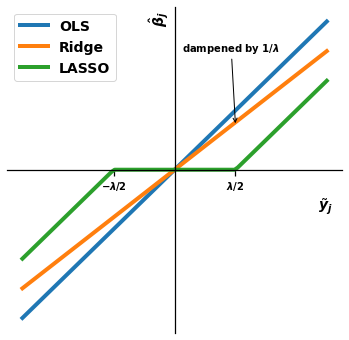
\includegraphics[width=.5\linewidth]{./results/ols-ridge-lasso-comp.png}
	\caption{The effect of shrinking the coefficient estimates in Ridge and LASSO regression methods compared to OLS for the simple approximation $\mathbf{\tilde{y}} = \mathbf{I\hat{\beta}}$. We see that Ridge will try to dampen $\hat{\beta}_1$ to reduce $\tilde{y}$'s variance, while LASSO drives $\hat{\beta}_1$ to zero when it becomes sufficiently small.}
	\label{fig:ols-ridge-lasso-comp}
\end{figure}

\subsection{The Design Matrix}
We want to approximate the Franke function, given by
\begin{equation}
\label{franke}
\begin{aligned}
f(x,y) &= \frac{3}{4}\exp{\left(-\frac{(9x-2)^2}{4} - \frac{(9y-2)^2}{4}\right)}+\frac{3}{4}\exp{\left(-\frac{(9x+1)^2}{49}- \frac{(9y+1)}{10}\right)} \\
&+\frac{1}{2}\exp{\left(-\frac{(9x-7)^2}{4} - \frac{(9y-3)^2}{4}\right)} -\frac{1}{5}\exp{\left(-(9x-4)^2 - (9y-7)^2\right) }.
\end{aligned}
\end{equation}
A $p$th degree polynomial in two variables $p_p(x,y) = 1 + x + y + x^2 + xy + y^2 ...$ can be used to approximate any function in two variables, such as the Franke function. We begin by collecting $n$ uniformly distributed random samples of the function $\mathcal{L}_{Franke} = \{(f(x_i, y_i), (x_i, y_i), i=0,1,...,n-1\}$. We first install the response variables (the $y_i$s) in a vector $\mathbf{y} \in \mathbb{R}^n$. Then we set up our \textit{design matrix} $\mathbf{X} \in \mathbb{R}^{n \times (p+1)}$ containing our predictors by evaluating each of the $p+1$ terms in $p_p(x_i,y_i)$ and install them in row $i$ of $\mathbf{X}$:
\begin{equation}
\mathbf{x}_i = [1 \quad x_i \quad y_i \quad x_i^2 \quad xy \quad y_i^2 \quad \cdots].
\end{equation}

The next step is then to solve $\mathbf{y} = \mathbf{X\beta} + \mathbf{\epsilon}$ to obtain the optimum coefficient estimates $\mathbf{\hat{\beta}}$ with the constraints given by the linear regression method's cost function. In order not to unfairly penalize Ridge and LASSO's coefficient estimates due to the value of the predictors, we must standardize them, that is; give each of $\mathbf{X}$'s columns a standard deviation of one. We do this by dividing each of the columns by its standard deviation \cite{james2013introduction}. Also, to account for the intercept, we will center all except the first of $\mathbf{X}$'s columns by subtracting its mean.

\subsection{The OLS Regression Method}
The ordinary least square's cost function $C_{OLS}(\mathbf{X},\mathbb{\beta})$ in equation (\ref{cost-ols}) has a closed form solution for obtaining the optimum coefficient estimates given by
\begin{equation}
\label{osl-reg}
	\mathbf{\hat{\beta}} = (\mathbf{X}^\intercal \mathbf{X})^{-1} \mathbf{X}^\intercal \mathbf{y}.
\end{equation}
See \cite{van2015lecture} for a thorough outline. Since $\mathbf{X}^\intercal \mathbf{X}$ may be uninvertible, we will use singular value decomposition $\mathbf{X} = \mathbf{U \Sigma V}^\intercal$ to calculate the pseudoinverse $\mathbf{X}^+ = \mathbf{V \Sigma}^{-1} \mathbf{U}^\intercal$, and then solve (\ref{osl-reg}) by $\mathbf{\hat{\beta}} = \mathbf{X}^+ \mathbf{y}$. See \cite{lay2016linear}.

Let us first use the OLS method on some randomly drawn samples from the Franke function (\ref{franke}), where we have added some normally distributed noise, $\epsilon$. We see in Figure \ref{fig:ols-simple-varying-n} that the variance in the approximation improves dramatically with increasing number of samples. This is explained by the decreased variance in the coefficient estimates, and we can illustrate this by plotting the confidence interval for each coefficient. As seen in Figure \ref{fig:ols-ci95}, for higher number of samples, the 95 \% confidence interval shrinks, meaning that the range around the estimated coefficient $\hat\beta_j$ in which the true unknown coefficients $\beta_j$ lays is narrowed \cite{james2013introduction}. The confidence interval is calculated by
\begin{equation}
\label{ci}
	\mathrm{CI_{95}^{(j)}}: \hat{\beta}_j \pm \mathrm{Var}(\hat{\beta}_j) \quad \text{where} \quad \mathrm{Var}(\hat{\beta}_j) = \sigma^2\sqrt{[(\mathbf{X}^\intercal \mathbf{X})^{-1}]_{jj}}.
\end{equation}
In the last term, due to \cite{fys-stk4155-notes}, $\sigma^2 = \mathrm{Var}(\epsilon)$, which is known and set to 0.05 in this example.

\begin{figure}[!htb]
	\centering
	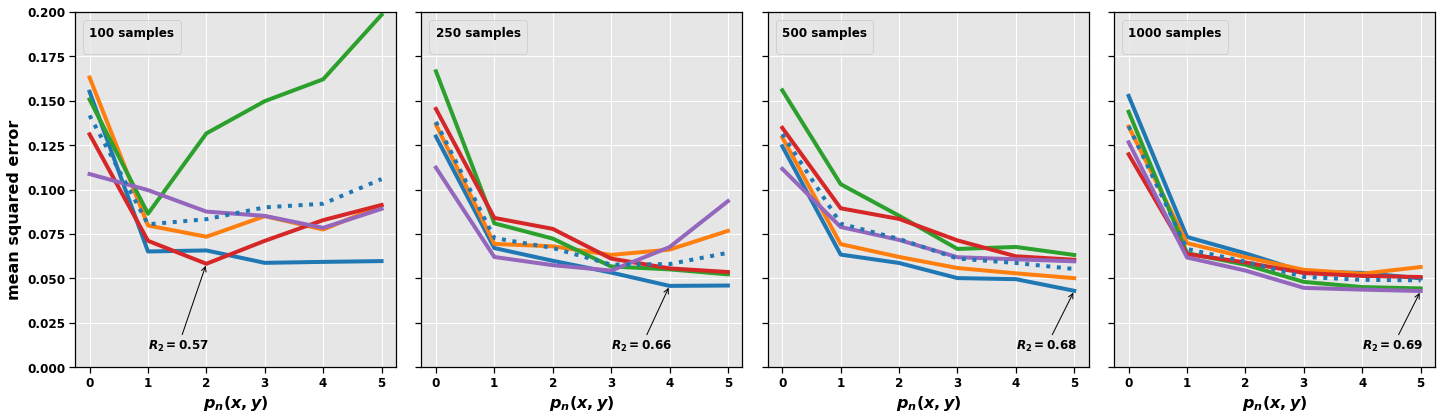
\includegraphics[width=1\linewidth]{./results/ols-simple-varying-n.png}
	\caption{Some approximations to the Franke function (\ref{franke}) with added noise $\epsilon  \sim \mathcal{N}(0, 0.05)$ for 100, 250, 500 and 1000 samples. Train-test split is 70/30 in all cases. Each curve represents a recalculation the estimated coefficients $\mathbf{\hat{\beta}}$ for a new randomly drawn data set. We see that the variance in the approximation decreases with increasing number of samples. The dotted blue line is the average.}
	\label{fig:ols-simple-varying-n}
\end{figure}

\begin{figure}[!htb]
\centering
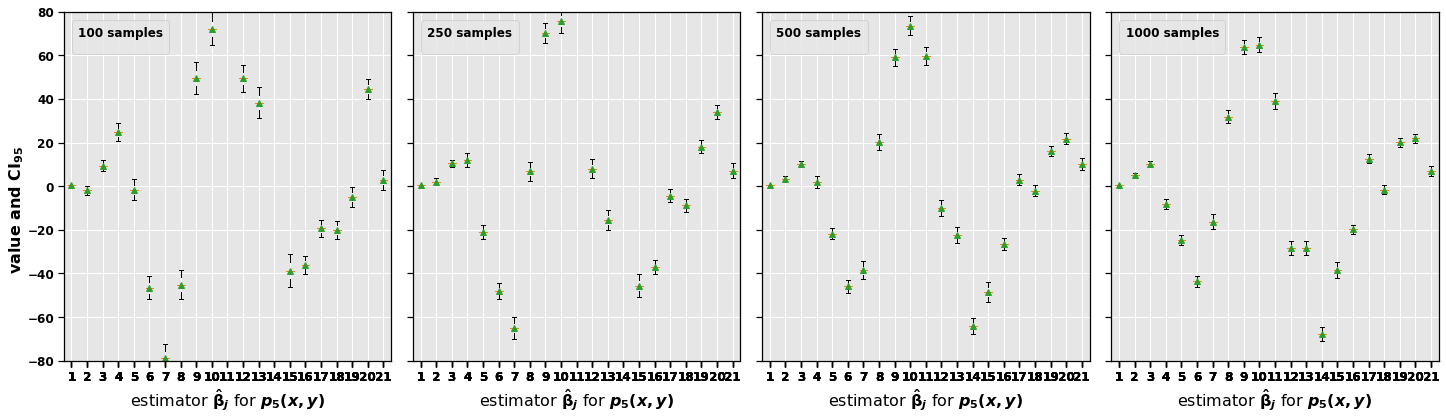
\includegraphics[width=1\linewidth]{./results/ols-ci95.png}
\caption{95 \% confidence interval ($\mathrm{CI_{95}}$) for the coefficient estimators $\hat{\beta}_j$ of $p_5(x,y)$ approximating the Franke function (\ref{franke}) with 100, 250, 500 and 1000 randomly drawn samples. Added noise is $\mathbf{\epsilon} \sim \mathcal{N}(0, 0.05)$ and the intervals are calculated using equation (\ref{ci}). We see that $\mathrm{CI_{95}^{(j)}}$ narrows for increasing number of samples, which is reflected in decreased $\mathrm{Var}(\tilde{y}_j)$. (See Figure \ref{fig:ols-simple-varying-n}).}
\label{fig:ols-ci95}
\end{figure}

Figure \ref{fig:ols-simple-varying-n} above illustrates the importance of re-sampling in linear regression model evaluation. Especially for the 100 and 250 samples, it is difficult to draw any conclusion about the suitability of the model, but if we look at the average (dotted blue line), we get a result which is easier to interpret. From the 100-sample results, we should expect best performance for a first-order polynomial $p_1(x,y)$ \textit{on average}, while for the 250-sample results, $p_3(x,y)$ seems to be best. For 500 and 1000, the results suggest that we could try to increase the model complexity beyond $p_5(x,y)$. Two more methodical ways re-sampling are Bootstrap and cross validation.

In Bootstrap re-sampling we split the data into a training and a test set, usually keeping 2/3 to 4/5 of the samples for training \cite{assignment}. Then, assuming the training set has $m$ samples, we collect from it the same number $m$ samples \textit{with} replacement, and calculate from those our coefficient estimates. Then we evaluate the model fit using the test data, note the result, and repeat the process for a number of times depending on the data set.

In $k$-fold cross-validation we also split the data into a training and a test set, but they are not fixed as for Bootstrap. Instead, we split the data into $k$ equally sized parts, keep one of the $k$ parts for test and train our model on the rest. Then we evaluate the model fit, note the result, and re-sample by picking the next of the $k$ parts, and handing the already tested part back to the training set. The process is repeated $k$ times (5-10 times in \cite{assignment}) so that all of the data has been tested once.

In Figures \ref{fig:ols-bootstrap} and \ref{fig:ols-cv} we see again the error estimates for the Franke function, but this time estimated with Bootstrap and cross validation re-sampling, respectively. Note that the scaling is different, so that even if the shape of the curves are similar, the actual error presented by Bootstrap in the overfitting region is at least a factor 10-100 larger than for cross validation. However, for the best fit, they both largely estimate the irreducible error $\sigma^2$ correctly (blue-shaded area) on the 500- and 1000-sample sets. On the 100- and 250-sample sets, however, there is a marked overestimation by Bootstrap. It is also worth to note that for the 100- and 250-sample sets, the best fit for the test data is achieved approximately when the training fit enters the irreducible error area.

Figure \ref{fig:ols-bootstrap} also presents the estimated bias-variance trade-off. We see that as expected, variance increases with model complexity, while bias decreases up to a point where high complexity itself makes the model biased.

Lastly, we note that the choice of $k$ does not seem to influence the results greatly for cross validation on this data set. We will use this to limit our scope when we do a similar evaluation of Ridge and LASSO further down.

\begin{figure}[!htb]
	\centering
	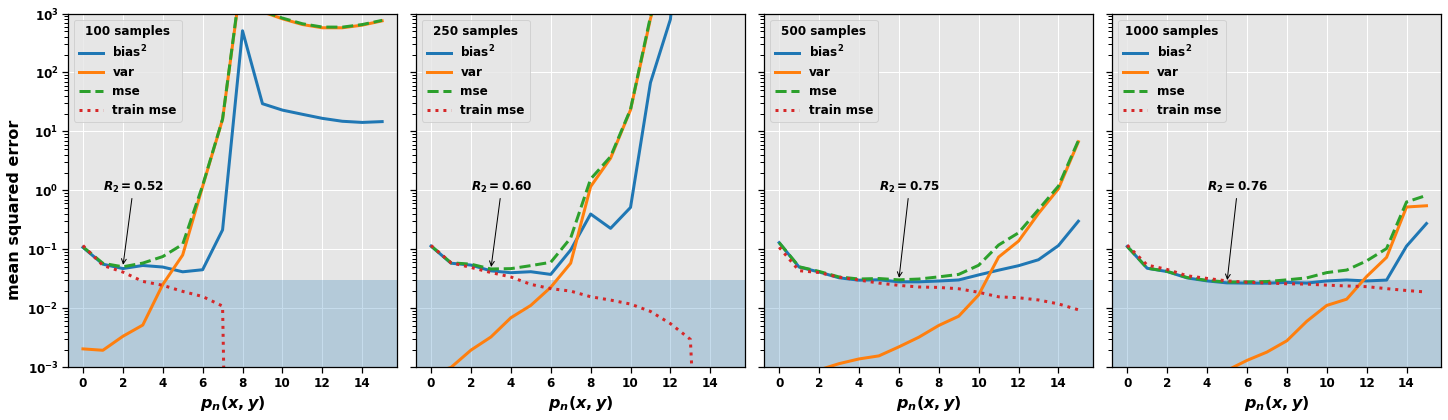
\includegraphics[width=1\linewidth]{./results/ols-bootstrap.png}
	\caption{Estimated error for the OLS polynomial fit to the Franke function (\ref{franke}) with 100, 250, 500 and 1000 samples and Bootstrap re-sampling. Added noise is $\mathbf{\epsilon} \sim \mathcal{N}(0, 0.03)$, indicated by the blue-shaded area. $\mathbf{X}$ has been centered, but not scaled. The estimates are calculated with a train-test split of 70/30 and with 25 bootstraps. We see that for the 500- and 1000-sample sets, the model estimates the irreducible error $\sigma^2$ well, while for the 100- and 250-sample sets it overestimates it. Cross validation performs a little better in this area. See Figure \ref{fig:ols-cv}. Concerning bias-variance trade-off, we see that as expected, for all data sets variance increases with increasing model complexity, while bias is reduced until complexity itself makes the model biased.}
	\label{fig:ols-bootstrap}
\end{figure}

\begin{figure}[!htb]
	\centering
	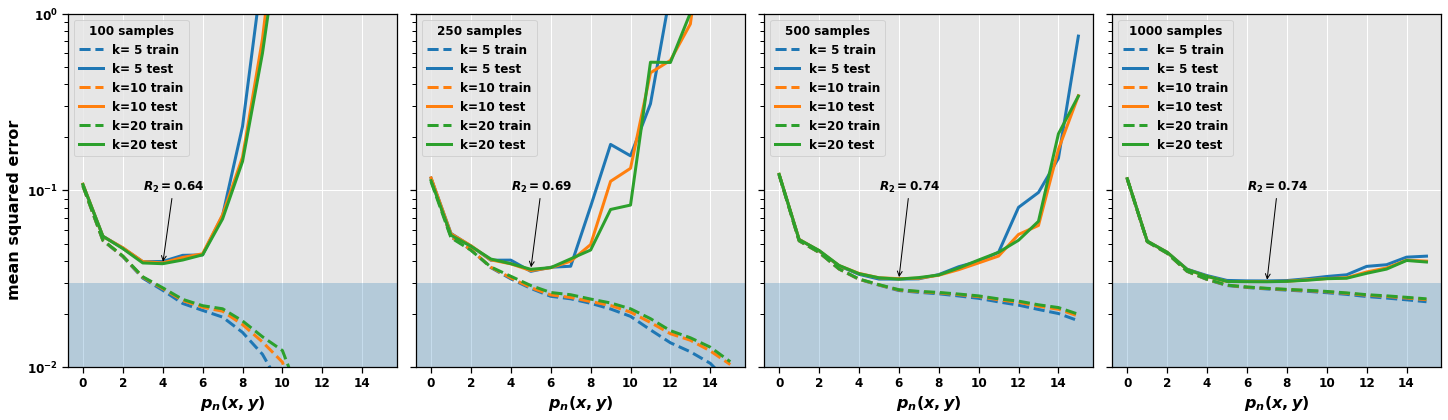
\includegraphics[width=1\linewidth]{./results/ols-cv.png}
	\caption{Estimated error for the OLS polynomial fit to the Franke function (\ref{franke}) with 100, 250, 500 and 1000 samples and $k$-fold cross validation re-sampling. Added noise is $\mathbf{\epsilon} \sim \mathcal{N}(0, 0.03)$, indicated by the blue-shaded area. $\mathbf{X}$ has been centered, but not scaled. The estimates are calculated with $k$s 5, 10 and 20. We see that the choice of $k$ does not influence the estimates except for in the overfitted area. For the 500- and 1000-sample sets, the model estimates the irreducible error $\sigma^2$ well, while for the 100- and 250-sample sets it overestimates it, but less so than does Bootstrap, though. See Figure \ref{fig:ols-bootstrap}.}
	\label{fig:ols-cv}
\end{figure}

\subsection{The Ridge Regression Method}
We saw in equation (\ref{cost-ridge}) that Ridge's cost function $C_{Ridge}(\mathbf{X},\mathbb{\beta})$ introduces a penalty $\sum \lambda \beta_j^2$ on the coefficient estimates in order to reduce their variance. As with OLS, Ridge's cost function also has a closed form solution for obtaining the coefficient estimates:
\begin{equation}
\label{ridge-reg}
	\mathbf{\beta}(\lambda) = (\mathbf{X}^\intercal \mathbf{X} + \lambda \mathbf{I})^{-1} \mathbf{X}^\intercal \mathbf{y}.
\end{equation}
In contrast to the solution to OLS's cost function, due to the addition of $\lambda \mathbf{I}$ the matrix $(\mathbf{X}^\intercal \mathbf{X} + \lambda \mathbf{I})$ \textit{is} invertible, which eases its solution. Again, see \cite{van2015lecture} for a thorough outline. Performing singular value decomposition on $\mathbf{X}$ does reveal an interesting property of Ridge regression. As shown in \cite{murphy2012machine}, with $\mathbf{X} = \mathbf{U \Sigma V}^\intercal$ and $\mathbf{u}_j$ being the $j$th row of $\mathbf{U}$, we can write equation (\ref{ridge-reg}) as
\begin{equation}
	\mathbf{\beta}(\lambda) = \sum_{j=1}^{p} \mathbf{u}_j \frac{\sigma_j^2}{\sigma_j^2 + \lambda} \mathbf{u}_j ^\intercal \mathbf{y}.
\end{equation}
This shows that introduction of the $\lambda$ term in Ridge's cost function (\ref{cost-ridge}) dampens or shrinks the coefficient estimates $\mathbf{\beta}$. See Figure \ref{fig:ols-ridge-lasso-comp} again for an illustration of this.

Even if we have a closed form solution to equation (\ref{ridge-reg}), finding the \textit{optimum} solution $\mathbf{\hat{\beta}} = \mathbf{\beta}(\hat{\lambda})$ must be done by trial and error. Figures \ref{fig:ridge-bootstrap} and \ref{fig:ridge-cv} show plots of searches for $\hat{\lambda}$ using Bootstrap and $k$-fold cross validation resampling, respectively. We see that both methods estimate the error well, but that cross validation only needs 500 samples for an exact approximation of the irreducible error $\sigma^2$, whereas Bootstrap needs 1000 (blue-shaded area). They both find the best fit for $p_5(x,y)$, all though for slightly different $\lambda$ value. MSE remains more or less unaffected by model complexity after that. For the other data sets, we see again as we saw for OLS that cross validation has better estimates than Bootstrap, even if the differences are less pronounced this time.

Figure \ref{fig:ridge-bootstrap} shows how Ridge operates: Increasing $\lambda$ forces the variance in the response $\mathrm{Var}(\mathbf{\tilde{y}})$ down, with a corresponding cost to bias. At the optimum point, $\hat{\lambda} = 3.09 \cdot 10^{-5}$ here, this trade-off reaches a best-ratio, which we select to fit our model.

\begin{figure}[!htb]
	\centering
	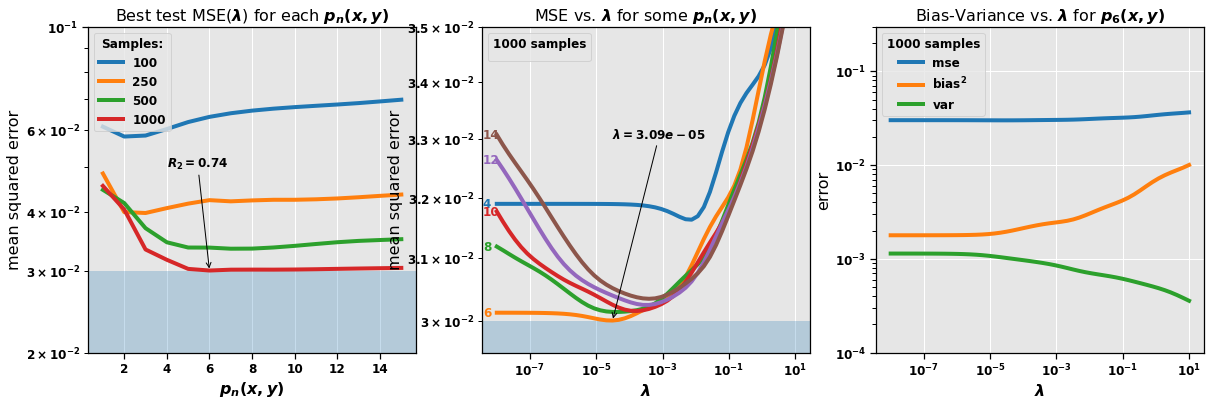
\includegraphics[width=1\linewidth]{./results/ridge-bootstrap.png}
	\caption{Estimated error for the Ridge polynomial fit to the Franke function (\ref{franke}) with 100, 250, 500 and 1000 samples and Bootstrap re-sampling. Added noise is $\mathbf{\epsilon} \sim \mathcal{N}(0, 0.03)$, indicated by the blue-shaded area. $\mathbf{X}$ has been centered and scaled. The estimates are calculated with a train-test split of 70/30 and with 25 bootstraps. To the left we see that we see that severe overfitting is prevented in all cases. For the 1000-sample set, the model estimates the irreducible error $\sigma^2$ accurately at around $p_5(x,y)$ and it remains very stable for increasing model complexity. The 500-sample set has a slight overfit beginning at around $p_{10}(x,y)$, but the error approximation is still good. The 250-sample set overestimates $\sigma^2$ by about 33 \%, but has about the same level of overfitting as the 500-sample set. The 100-sample has a best approximation of about $2\sigma^2$. Cross validation performs a better for small data sets. See Figure \ref{fig:ridge-cv}. To the right we see the bias-variance trade-off depending on $\lambda$. Increasing $\lambda$ reduces the variance in the response, which comes with a cost in bias, as expected from Ridge.}
	\label{fig:ridge-bootstrap}
\end{figure}

\begin{figure}[!htb]
	\centering
	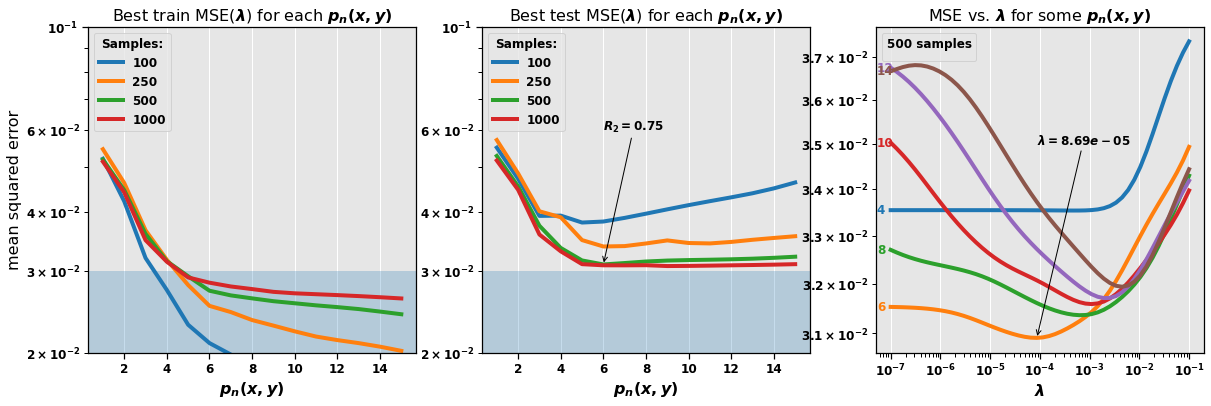
\includegraphics[width=1\linewidth]{./results/ridge-cv.png}
	\caption{Estimated error for the Ridge polynomial fit to the Franke function (\ref{franke}) with 100, 250, 500 and 1000 samples and 5-fold cross validation re-sampling. Added noise is $\mathbf{\epsilon} \sim \mathcal{N}(0, 0.03)$, indicated by the blue-shaded area. $\mathbf{X}$ has been centered and scaled. To the left we see that the train MSE indicates heavy overfitting, but in the middle that Ridge prevents severe overfitting in all test cases. For the 500-sample set, the model estimates the irreducible error $\sigma^2$ accurately at $p_5(x,y)$ and that it has a slight overfit after that, but the error approximation is still good. The 1000-sample remains approximation remains very stable for increasing model complexity. The 250-sample set overestimates $\sigma^2$ only by about 10 \%, and has about the same level of overfitting as the 500-sample set. The 100-sample overestimates $\sigma^2$ by about 33 \%. Overall, cross validation performs better than Bootstrap on this data set. See Figure \ref{fig:ridge-bootstrap}. To the right we see test MSE as a function of $\lambda$ for the 500-sample approximations.}
	\label{fig:ridge-cv}
\end{figure}

\subsection{The LASSO Regression Method}
We saw in equation (\ref{cost-lasso}) that like Ridge's cost function, LASSO's cost function $C_{LASSO}(\mathbf{X},\mathbb{\beta})$ introduces a penalty $\sum \lambda |\beta_j|$ on the coefficient estimates in order to reduce their variance. In contrast to Ridge, and OLS for that matter, LASSO's cost function does not have a closed form solution, meaning that for each $\lambda$ we must search both for a solution that minimizes the cost function itself. In this report we will use \lstinline|sklearn.linear_model.Lasso| in Python's \lstinline|scikit-learn| module to search for this solution.

Figures \ref{fig:lasso-bootstrap} and \ref{fig:lasso-cv} show plots of searches for $\mathbf{\hat{\beta}}, \hat{\lambda}$ using Bootstrap and $k$-fold cross validation resampling, respectively. Again, we see that both methods estimate the irreducible error almost equally well for the larger data sets, while cross validation is a little more stable for smaller data sets. The bias-variance trade-off, seen to the right in Figure \ref{fig:lasso-bootstrap}, behaves as we expect, with increased $\lambda$ reducing the variance in the response $\mathrm{Var}(\mathbf{\tilde{y}})$. This comes of course with a cost in model bias.

\begin{figure}[!htb]
	\centering
	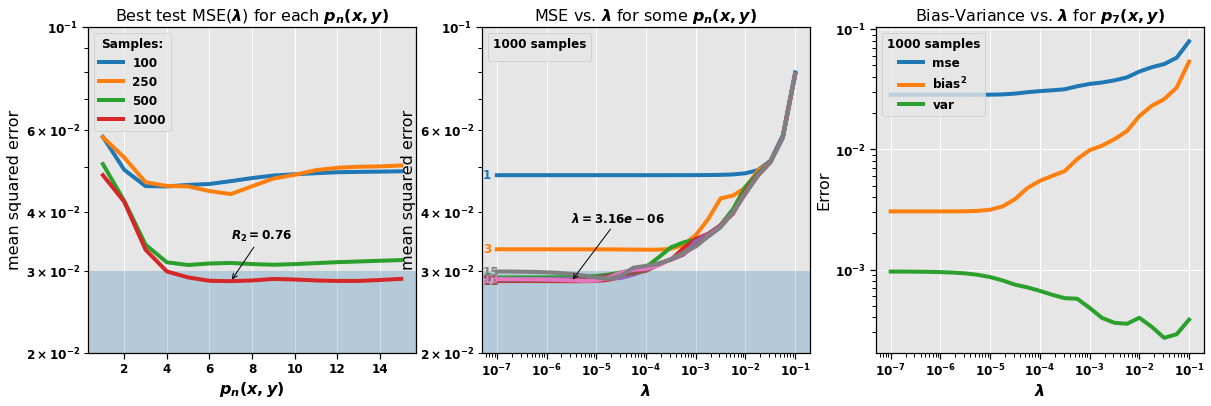
\includegraphics[width=1\linewidth]{./results/lasso-bootstrap.png}
	\caption{Estimated error for the LASSO polynomial fit to the Franke function (\ref{franke}) with 100, 250, 500 and 1000 samples and Bootstrap re-sampling. Added noise is $\mathbf{\epsilon} \sim \mathcal{N}(0, 0.03)$, indicated by the blue-shaded area. $\mathbf{X}$ has been centered and scaled. The estimates are calculated with a train-test split of 70/30 and with 25 bootstraps. To the left we see that severe overfitting is prevented in all cases. For the 1000-sample set, the model estimates the irreducible error $\sigma^2$ fairly well at around $p_4(x,y)$ and it remains very stable for increasing model complexity. It may seem a little strange that the fit in this case is \textit{better} than $\sigma^2$, but this comes from the randomness of the test set samples, indicating that they are ever so slightly off-center. Repeating the experiment with a different test set could yield a best fit slightly above the line. The 500-sample approximation performs almost equally well as the 1000-sample approximation, and show no sign of overfitting. The 100- and 250-sample sets overestimates $\sigma^2$ by about 50 \%, and show slight signs of overfitting. Bootstrap performs somewhat better than cross validation on smaller data sets, and worse on larger. See Figure \ref{fig:lasso-cv}. To the right we see the bias-variance trade-off depending on $\lambda$. Increasing $\lambda$ reduces the variance in the response, which as we see comes with a quite significant cost in bias, leading to a relatively small $\hat{\lambda}$. \lstinline|scikit-learn Lasso()| options: \lstinline|\{'max_iter':1E4, 'fit_intercept':False, 'tol':.001\}|}
	\label{fig:lasso-bootstrap}
\end{figure}

\begin{figure}[!htb]
	\centering
	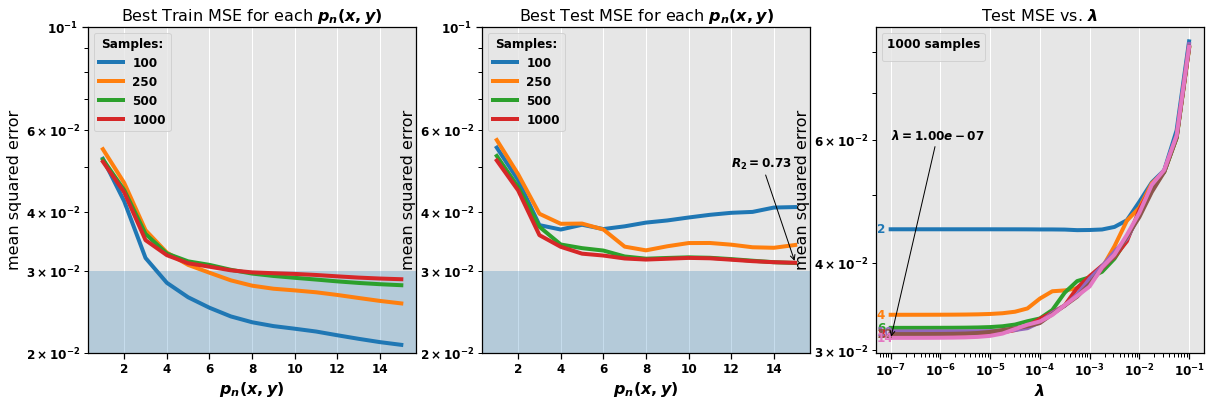
\includegraphics[width=1\linewidth]{./results/lasso-cv.png}
	\caption{Estimated error for the LASSO polynomial fit to the Franke function (\ref{franke}) with 100, 250, 500 and 1000 samples and 5-fold cross validation re-sampling. Added noise is $\mathbf{\epsilon} \sim \mathcal{N}(0, 0.03)$, indicated by the blue-shaded area. $\mathbf{X}$ has been centered and scaled. To the left we see that the train MSE indicates heavy overfitting, but in the middle that LASSO prevents severe overfitting in all test cases. For the 500- and 1000-sample sets, the model estimates the irreducible error $\sigma^2$ quite accurately at $p_5(x,y)$ and do not show any overfitting after that. Increasing model complexity beyond $p_{15}(x,y)$ did not improve the $R^2$ value when that was tested (not shown). The 250-sample set also estimates $\sigma^2$ well at $p_8(x,y)$, before it gets a slight overfit. The 100-sample overestimates $\sigma^2$ by about 20 \% at $p_4(x,y)$, and then. Bootstrap performs somewhat better than cross validation on smaller data sets, and worse on larger. See Figure \ref{fig:lasso-bootstrap}. To the right we see test MSE as a function of $\lambda$ for the 1000-sample approximations. \lstinline|scikit-learn Lasso()| options: \lstinline|\{'max_iter':1E4, 'fit_intercept':False, 'tol':.01\}|}
	\label{fig:lasso-cv}
\end{figure}

\clearpage
\section{Results} \label{results}
% - Present your results
% - Give a critical discussion of your work and place it in the correct context.
% - Relate your work to other calculations/studies
% - An eventual reader should be able to reproduce your calculations if she/he wants to do so. All input variables should be properly explained.
% - Make sure that figures and tables should contain enough information in their captions, axis labels etc so that an eventual reader can gain a first impression of your work by studying figures and tables only.
To finish our qualitative evaluation of the OLS, Ridge and LASSO regression methods, lets first look at what each of them do to the coefficient estimates $\hat{\beta}_j$ when we do the polynomial fit to the Franke function (\ref{franke}). After that we will evaluate their performance on \textit{real} data, altitude levels of a mountain range.

\subsection{OLS, Ridge and LASSO Coefficient Estimates}
We expect that Ridge shall \textit{shrink} the coefficients more or less evenly, but not all the way to zero as we expect LASSO to do, since LASSO shall also pick those predictors that best explain $\mathbf{f}(\mathbf{X})$, and preferably drive the rest to zero. In addition, and as a consequence of this, we expect that the variance shall be greatly reduced, and more so for LASSO than Ridge, since it is more agressive. 

Figure \ref{fig:ols-ridge-lasso-betas} shows the coefficient estimates $\hat{\beta}_j$ for OLS, Ridge and LASSO when fitting $p_6(x,y)$ to the Franke function with 1000 samples. $\lambda$s are chosen to give the best fit, according to our evaluation with cross validation above in Figures \ref{fig:ridge-cv} and \ref{fig:lasso-cv}. We see that indeed, the Ridge and LASSO do reduce the values of the estimates, and the variance is also reduced. In both cases also more aggressively for LASSO than for Ridge. However, with this model on this data set LASSO does not drive any of the coefficient estimates to zero, so we cannot derive some underlying truth about $\mathbf{f}(\mathbf{X})$ from them here, which may be reasonable since OSL's fit is just as good as Ridge and LASSO's for this model complexity.

\begin{figure}[!htb]
	\centering
	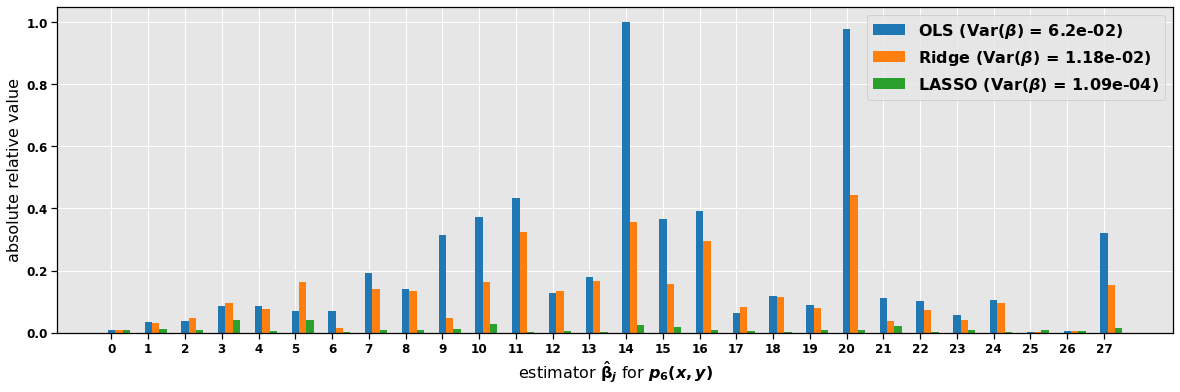
\includegraphics[width=1\linewidth]{./results/ols-ridge-lasso-betas.png}
	\caption{OLS, Ridge and LASSO coefficient estimates $\hat{\beta}_j$ when fitting $p_6(x,y)$ to the Franke function with 1000 random samples and noise $\mathbf{\epsilon} \sim \mathcal{N}(0, 0.03)$. $\lambda$ values for Ridge and LASSO are chosen to give the best fit, as found in the cross validation evaluation: $\lambda_{Ridge} = 8.7 \cdot 10^{-5}$; $\lambda_{LASSO} = 3.2 \cdot 10^{-6}$. We see that LASSO shrinks the estimates more aggressively than does Ridge, and that $\mathrm{Var}(\mathbf{\hat{\beta}})$ follows the same pattern. However, none of LASSO's coefficients are driven to zero.}
	\label{fig:ols-ridge-lasso-betas}
\end{figure}

\subsection{Geological Data: Comparison of the OLS, Ridge and LASSO Regression Methods}
We will now investigate the performance of each of the regression methods on a highly irregular data set. The data set represents the altitude above sea level of a mountain range in the central United States, collected from \cite{geo-data}. See Figure \ref{fig:geo-data}, left part. The data has unknown quality; that is, the irreducible error level $\sigma^2$ is unknown. We will however assume that the error is normally distributed with zero mean, such that the data again can be represented as in equation (\ref{y_f_eps}), repeated here for convenience:
\begin{equation*}
\mathbf{y} = \mathbf{f}(\mathbf{X}) + \mathbf{\epsilon} \quad \text{, where} \quad \mathbf{f}(\mathbf{X}) = \mathbf{X} \mathbf{\beta} \quad \text{and} \quad \mathbf{\epsilon} \sim \mathcal{N}(0, \sigma^2).
\end{equation*}

The data set contains $3601 \times 3601 \approx 13$ million data points, which is prohibitively large. We therefore draw uniformly distributed random samples from the data set to form subset of $n$ samples which we do our study on, as for the Franke function. Figure \ref{fig:geo-ols-cv} shows that the noise level $\sigma^2$ probably lies a little bit above $3 \cdot 10^{-3}$, and that using a larger data set than 5000 samples does not bring any benefits with regards to model fit parameter $R^2$, so we will base our study on 5000 samples.

Ridge regression on the 5000-sample data set give slightly worse fit, as we see in Figure \ref{fig:geo-ridge-cv}. The model $R^2$ is only 0.80, compared to 0.83 for simple OLS, and this on the 30th polynomial, as opposed to the 20th for OLS. We see that $\hat{\lambda}$ for the Ridge's $p_{30}(x,y)$ is very small at $3.7 \cdot 10^{-10}$, indicating that there is not much variance in the response for Ridge to trade off against model bias in this data set. Beyond this level, it might be numerical instability which causes the estimates to increase.

Figure \ref{fig:geo-lasso-cv} shows the results for LASSO regression on the same data set. We see that the fit is markedly worse than both Ridge and OLS. $R^2$ fit is only 0.71 at the 30th polynomial, but as we see the trend suggests that it would be possible to achieve at least some improvement to the fit. As for Ridge, $\hat{\lambda}$ for the best polynomial $p_{30}(x,y)$ is small, but stabilizing at around $1.0 \cdot 10^{-7}$. Again as for Ridge, this suggests that the data set does not offer the opportunity to trade bias against variance.

In Figure \ref{fig:geo-data}, we see how the three approximations reproduces the original data set. For OLS and, if to a lesser extent, also for Ridge, we clearly see the main features are preserved, but that all smaller details disappears. For LASSO, the reproduction rather poor with all original features completely blurred.


\begin{figure}[!htb]
	\centering
	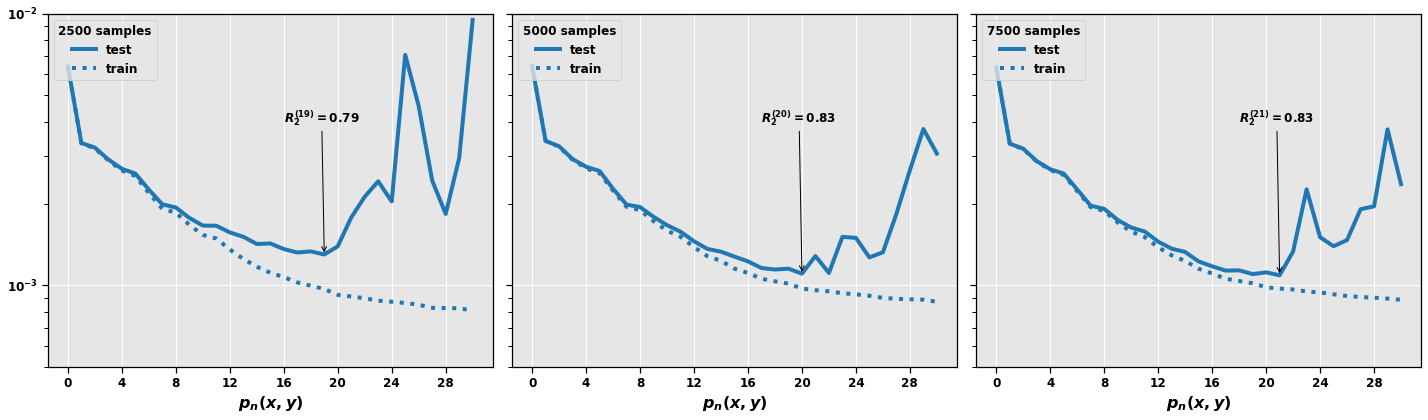
\includegraphics[width=1\linewidth]{./results/geo-ols-cv.png}
	\caption{OLS polynomial fit to geological data with 2500, 5000 and 7500 randomly selected samples. Error approximation by 5-fold cross validation. We see that the noise level probably lies a little bit above $3 \cdot 10^{-3}$, and that collecting more than 5000 samples does not give better fit for the polynomial. Hence, we base our evaluation of the suitability of OLS, Ridge and LASSO on the data set with 5000 samples.}
	\label{fig:geo-ols-cv}
\end{figure}

\begin{figure}[!htb]
	\centering
	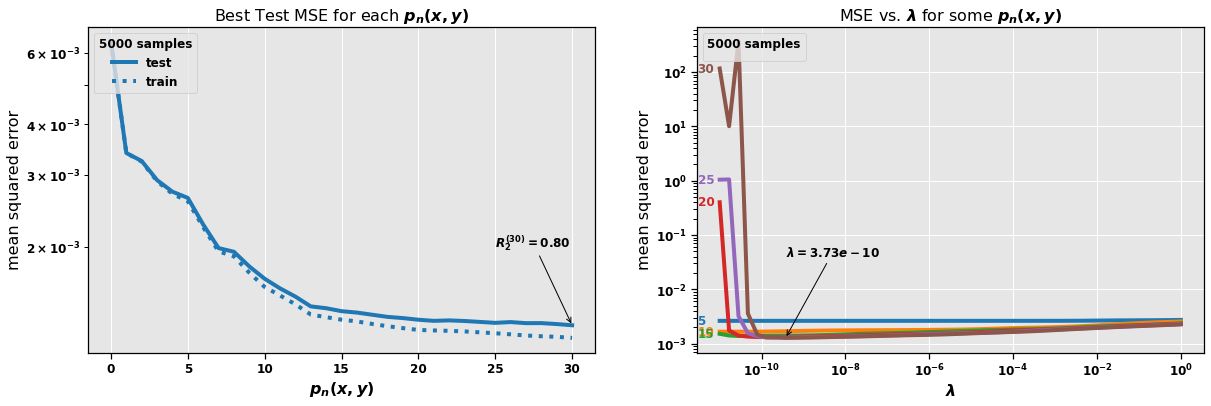
\includegraphics[width=1\linewidth]{./results/geo-ridge-cv.png}
	\caption{Ridge polynomial fit to geological data with 5000 randomly selected samples. Error approximation by 5-fold cross validation. Noise level approximated to about $3 \cdot 10^{-3}$ using OLS (see Figure \ref{fig:geo-ols-cv}). The model fit $R^2 = 0.80$ is markedly poorer than OLS and Ridge. The small $\hat{\lambda}$ for $p_{30}(x,y)$ suggests that bias-variance trade-off does not pay off greatly in this case.}
	\label{fig:geo-ridge-cv}
\end{figure}

\begin{figure}[!htb]
	\centering
	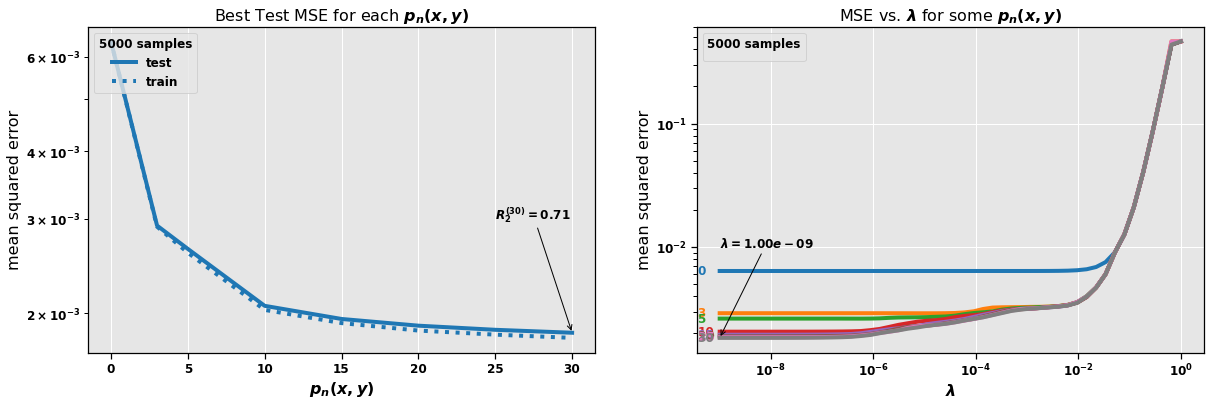
\includegraphics[width=1\linewidth]{./results/geo-lasso-cv.png}
	\caption{LASSO polynomial fit to geological data with 5000 randomly selected samples. Error approximation by 5-fold cross validation. Noise level approximated to about $3 \cdot 10^{-3}$ using OLS (see Figure \ref{fig:geo-ols-cv}). The model fit $R^2 = 0.71$ and very small $\hat{\lambda}$ for $p_{30}(x,y)$ suggests that bias-variance trade-off does not pay off greatly in this case. We see however that }
	\label{fig:geo-lasso-cv}
\end{figure}

\begin{figure}[!htb]
	\centering
	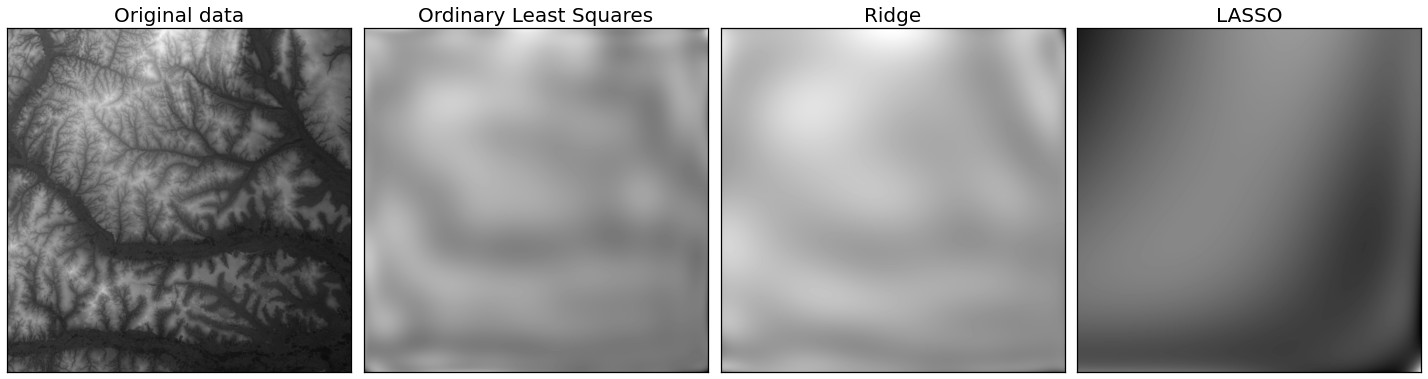
\includegraphics[width=1\linewidth]{./results/geo-data.png}
	\caption{To the left we see the original geological data reflecting altitude above sea level of a mountain range. The three images to the right are reproductions generated by solving the optimum $p_{n}(x_i,y_i)$ for $i \in [0,3600]$ obtained for each regression method OLS, Ridge and LASSO, respectively. OSL and Ridge reproduce the main features of the original, while LASSO's reproduction is completely unrecognizable.}
	\label{fig:geo-data}
\end{figure}

\clearpage
\section{Discussion and Conclusion} \label{conclusion}
% - State your main findings and interpretations
% - Try as far as possible to present perspectives for future work
% - Try to discuss the pros and cons of the methods and possible improvements
In the controlled case with the Franke function, we saw that the assumption that the data points $\mathbf{y}, \mathbf{X}$ could be represented by a linear function $\mathbf{f}(\mathbf{X}) = \mathbf{\beta X}$ with an error $\mathbf{\epsilon} \sim \mathcal{N}(0, \sigma^2)$. We then saw that the best-fit solution $\mathbf{\hat{\beta}}$ to the equation $\mathbf{y} = \mathbf{\beta X} + \mathbf{\epsilon}$, given the cost functions for either OLS, Ridge and LASSO lets us reproduce the underlying function $\mathbf{f}$ with high accuracy, and that we also obtain a precise estimate for the error $\sigma^2$ in the data.

The performance of the three regression methods appear to not be very dependent on whether we use Bootstrap of cross validation resampling if the data set is large enough, but for smaller data sets, cross validation performed best on the Franke data. This is good for two reasons; firstly that for this data it does not matter much which method we choose, and secondly because $k$-fold cross validation is faster than bootstrap since it runs through the data only 5 to 10 times, as opposed to 20 to 30 times for Bootstrap. Hence, cross validation is the method of choice here.

We have also seen that Ridge and LASSO with cross validation perform better than OLS on smaller data sets, where number of $n$ is not much greater than $p$. The reason for this is that these methods let us choose a model with higher complexity than OLS, since they remedy the high variance in the response $\mathrm{Var}(\mathbf{y})$ which would otherwise occur by penalizing large coefficient estimates and reducing their variance.

On the geological data, on the other hand, $n >> p$, which is ideal for OLS, since complexity can be increased without too high cost in variance, and the randomness in the test data will closely resemble that of the training data. As a result, OLS performs markedly better than Ridge here, and LASSO performs quite poorly, as we saw in the image reproduction in Figure \ref{fig:geo-data}.

Future expansion of this study should include more kinds of \textit{areally} distributed data, like fertility vs. location or income vs. a persons physical weight and height, to proper gauge where OLS, Ridge and LASSO each come to best use in these applications.

\clearpage
\bibliographystyle{plain}
\bibliography{project1.bib}
\end{document}
